\section{Problem Statement}

Ever since \textit{physarum polycephalum}, a.k.a "the Yellow slime mould", started being studied for its computational intelligence, it has garnered a great deal of attention in the world of biology-inspired computing with respects to network science, logic, path-finding, and many other applications in computing. This is due to the changing topology of the mycelial network as it explores its environment and searches for food, displaying many intelligent behaviors in the process. Sun has stated this intelligence can be exploited to solve various network optimization problems. Amongst other findings, experiments related to the slime mould confirm that it can optimize networks, solve mazes and generate a minimum spanning graph with use of its foraging mechanics \cite{rulesBioDesign} \cite{mazesolving}.

By 2018, a new research was published where Adamatzky proposed that Fungi Basidiomycetes are a better candidate for such experimentation than \textit{physarum polycephalum} \cite{fungalcomp} . This is due to the fact that the former is less susceptible to environmental factors, is easier to obtain and manipulate. He proposed that since both are analogous to each other, experiments done on \textit{physarum polycephalum} can be replicated using Mycelium networks from Fungi Basidiomycetes.

We aim to fill this space in the field of Bio-inspired computing by replicating with Mycelium networks, the Tokyo Rail Network experiment which was performed using \textit{physarum polycephalum} \cite{rulesBioDesign}. With the obtained results, we aim to produce an algorithm to mimic the foraging and growth pattern of Mycelium networks.

\section{Proposed Solution}

In order to be able to simulate the behavior of Mycelial networks we will have to analyze the behavior of it growth. Our system starts with the lab component beginning with obtaining the spores and isolating the most viable strain with relevance to weather and environmental condition. Once a viable strain is obtained we shall start observing the culture growth at timed intervals using images. These images are then to be processed using an image processing software called NEFI 2.0, this will then yeild us raw data in the form of a weighted undirected planar graph whih then we can analyse and work with. Using graph analysis tools such as MATLAB and NEFI 2.0 we will look into how this growth can be modelled mathematically and formulate an algorithm to represent the Mycelial behavior. This algorithm will then be tested alongside live cultures to see if it is representative of the mycelium behavior. Once confident, we aim to use this algorithm as a backbone to our simulation which we can then use to simulate mycelial networks and move to applying this optimizing algorithm to propose a viable subway transport network for Karachi.

\section{Intended User}

\paragraph{Agents with the potential to create an underground network}
\mbox{}\\
Since our experiment yields a hypothetical underground subway network within Karachi, we feel it will prove to be a pertinent asset to anyone equipped with 
the resources and potential to build such an underground network. 

\paragraph{Students of Computer Science}
\mbox{}\\
Students, such as those studying computational intelligence, may find our work helpful, when learning about biology-inspired computer algorithms.

\section{Project gantt chart and deliverables}
\begin{figure}
    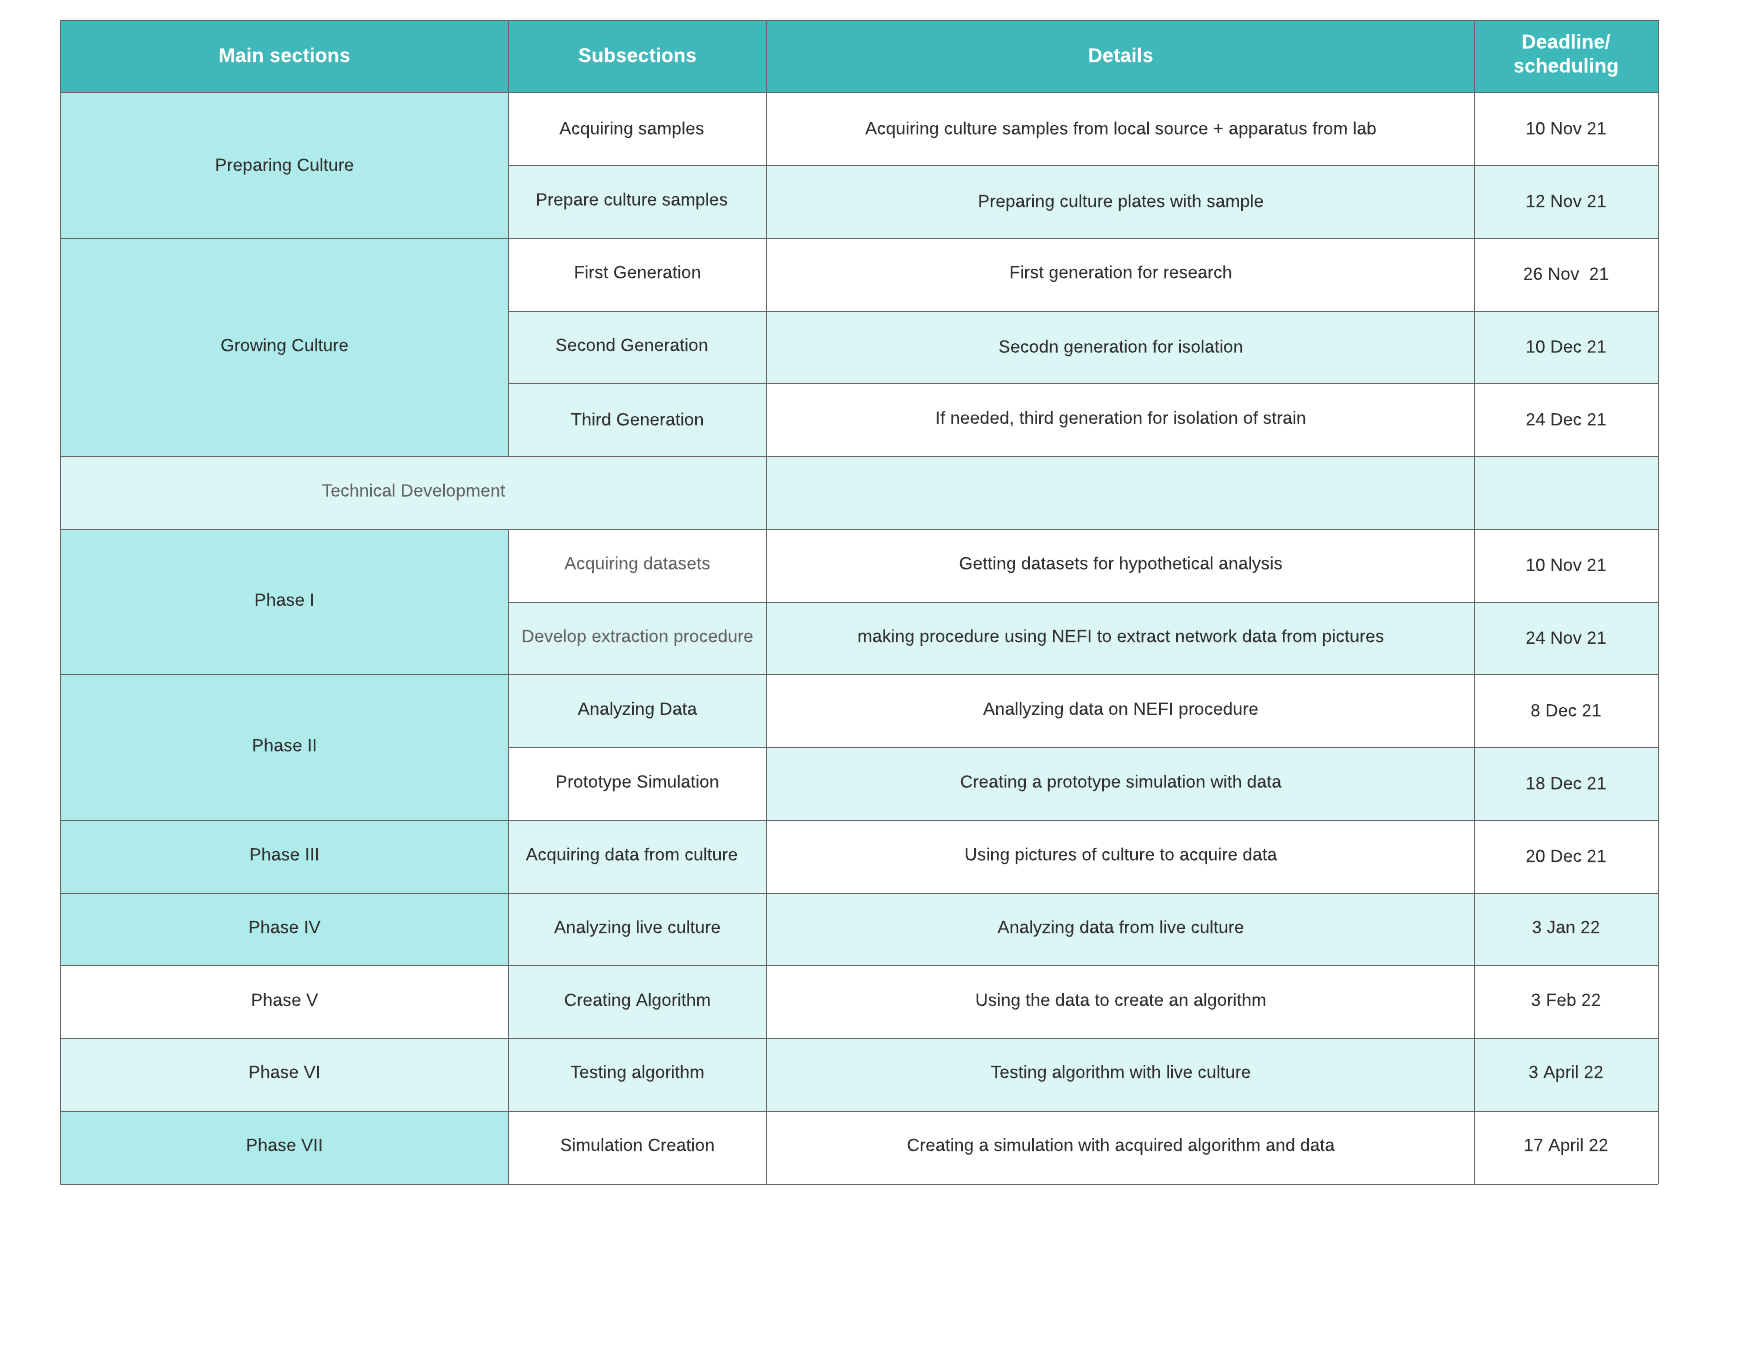
\includegraphics[scale=0.6]{Images/gantt_chart.png}
    \caption{Gantt Chart}
    \label{fig:gantt}
\end{figure}

Deliverables: The approach for our deliverables will be largely adapted from following the procedure for unraveling slime mould intelligence as outlined by Sun
\cite{steiner_tree}.
    
    \begin{enumerate}
        \item Perform experiments revealing mycelium intelligence on agar.
        \item Based on the experimental results, model the mycelium intelligence (algorithm design, heuristic methods, agent-based modelling, etc).
        \item Customize the model for our applications and develop front-end software for running the simulation of our model.
    \end{enumerate}
    
    Note that the approach outlined was for physarum-inspired networking models, but is generalizable to mycelium networks as well.
    
    The following SMART deliverables have been identified by our team:
    
    \begin{itemize}
        \item \textbf{A model of mycelium growth in a generalised environment:} The model will be based on the real behaviour of mycelium as it colonizes an agar plate in search of food. Algorithms, heuristic approach and agent-based models can all potentially be used in this model.
        \item \textbf{Front-end simulation application using the simulation over transport networks for Karachi:} The simulation should have several parameters that can be adjusted, including addition of nodes, changing terrain, and changing environmental conditions. An option for switching between slime mould and oyster mushroom mycelium may also be included in the simulation, to compare and contrast the behaviour of both organisms.
        \item \textbf{Viable mycelium cultures for experimentation in the lab:} Multiple strains will be obtained from grain spawn colonized on agar. From the isolated strains, the ones showing rapid growth, resistance to contamination and temperature fluctuations will be selected. The experiment will be repeated with several mycelium strains for accuracy of results.
        \item A 3D-printed, scaled down model of Karachi's map on an agar plate. This will be the model used for colonization and studying network optimization, as was done in previous experiments \cite{rulesBioDesign} \cite{slimeapprox}
        
    \end{itemize}

\section{Key Challenges}
The following are the key challenges, and their potential solutions (or precautionary measures that may help prevent them), identified by our team.

\paragraph{The Mycelium culture does not survive as long as required}
\mbox{}\\
Grow extra cultures in preparation.

\paragraph{Unforeseen circumstances cause delays in weekly deliverables.}
\mbox{}\\
Exaggerate goals and deadlines in documentation, to allow a buffer-level cushioning at any and every stage of the project.

\paragraph{Hit-by-a-bus Syndrome}
\mbox{}\\
All areas of the project, regardless of who is leading, will be inclusive of participation (and learning, if need be) from all team members. 

\paragraph{Acquiring Datasets}
\mbox{}\\
We plan on reaching out to the first authors of research papers which make use of the same (or similar) data as us, in hopes of acquiring their datasets. Additionally, we also plan to acquire images of a culture with timed intervals to obtain data that we need, using image processing.
